\documentclass[tikz,border=10mm]{standalone}
\begin{document}
	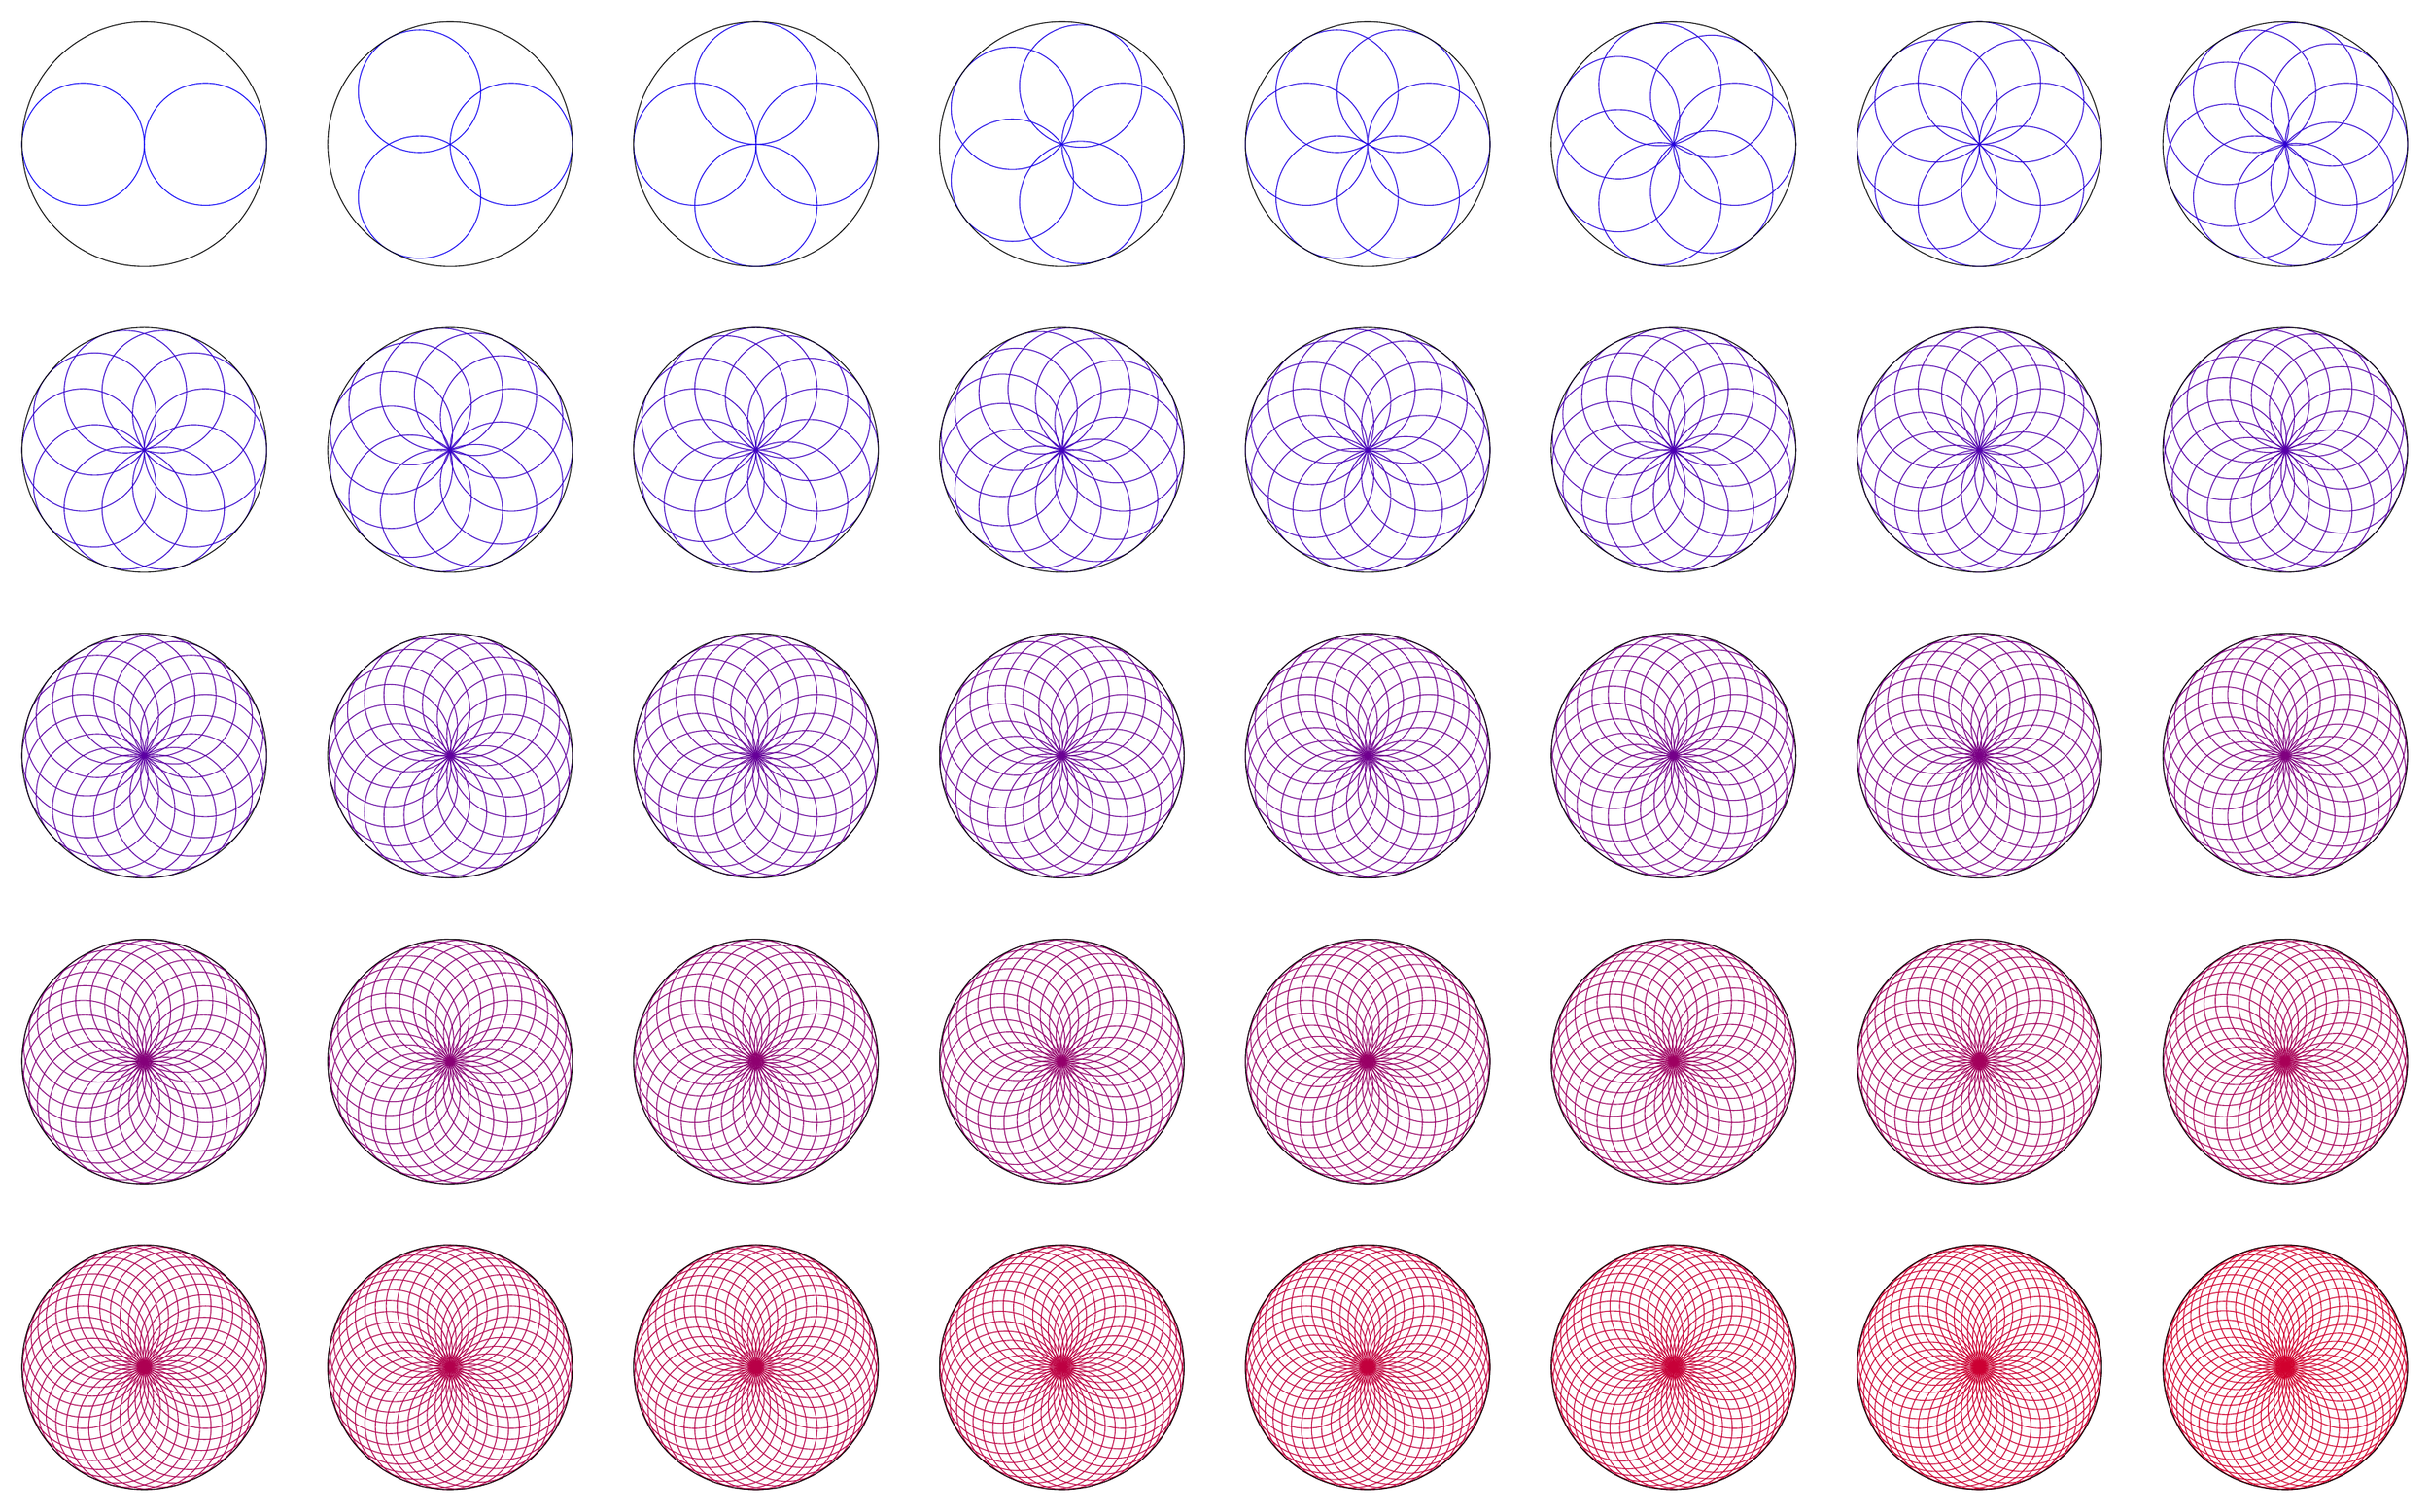
\begin{tikzpicture}
		\tikzset{little circle/.pic={
				\pgfmathsetmacro{\p}{2*#1}
				\foreach \i in {1,...,#1}
				\draw[red!\p!blue] ({\i*360/#1}:1) circle(1);
				\draw (0,0) circle(2);
		}}
		\newcounter{myLC}
		\setcounter{myLC}{1}
		\foreach \j in {1,...,5}
		\foreach \i in {1,...,8}{
			\stepcounter{myLC}
			\path (5*\i,-5*\j) pic{little circle=\themyLC};
		}
	\end{tikzpicture}
\end{document}